

\documentclass[colorlinks=true,pdfstartview=FitV,linkcolor=blue,
            citecolor=red,urlcolor=magenta]{ligodoc}

\usepackage{graphicx}
\usepackage{amssymb}
\usepackage{amsmath}
\usepackage{longtable}
\usepackage{rotating}
\usepackage[usenames,dvipsnames]{color}
\usepackage{fancyhdr}
\usepackage{subfigure}
\usepackage{hyperref}
\ligodccnumber{T}{11}{XXXXX}{}{vX}% \ligodistribution{AIC, ISC}

\usepackage{bmpsize}



\title { \large Devoloping Phase Map of Cavity Mirrors using Laser Mode Spectroscopy }

\author{\begin{center}Keerthana S Nair
\\{Mentors: Gautam Venugopal, Koji Arai and Rana Adhikari}\end{center}}


\begin{document}

\section{Abstract} 
This project is inspired by the summer projects done by Kaustubh Singhi and Naomi Wharton. The main goal of this project is to obtain a more precise and accurate cavity scan data and to develop a more reliable Phase/Mirror map of the cavity mirrors. This is only a project proposal, thus full details of the project is not provided. The idea of this article is just to set an outline for the project work.
\section{Introduction} 
\subsection{Gravitational Waves}
Einstein's general theory of relativity explains gravity as a distortion of spacetime caused by the presence of matter or energy. A massive object generates a gravitational field by warping the geometry of the surrounding spacetime. Due to some of the most violent and energetic processes in the universe the gravitational field around it varies with respect to time and this produces ripples in the fabric of space-time \cite {gravitational waves}. These ripples are known as the Gravitational Waves. Einstein's mathematics showed that the waves produced by massive accelarating objects like neutron stars or black holes will have sufficient energy to get radiated from the source. These ripples would travel at the speed of light through the Universe. The ripple carry information about their origin, as well as invaluable clues to the nature of gravity. Thus study of gravitational waves provide us better understanding of the existing Universe and also about the early universe shortly after the Big Bang. This emerging branch of Physics is known as the Gravitational-wave astronomy.A simulation of production of Gravitational waves from binary stars orbiting around each other is shown in Figure \ref{fig:gwave}. Even though the existence of Gravitational waves were first predicted in 1916, the first direct detection of Gravitational Waves occurred on September 14, 2015 using the Laser Interferometer Gravitational Observatory (LIGO). This work earned three scientist the 2017 Nobel Prize in Physics \cite{gwaveurl}.

%%If you need to cite a source, do it like this: \cite{CitationKeyWord}.

%%Pictures and figures are awesome!  You should include them wherever
%%they will help make something more clear, as you can see in Figure \ref{fig:gwave}.

 \begin{figure}[htbp]
\begin{center}
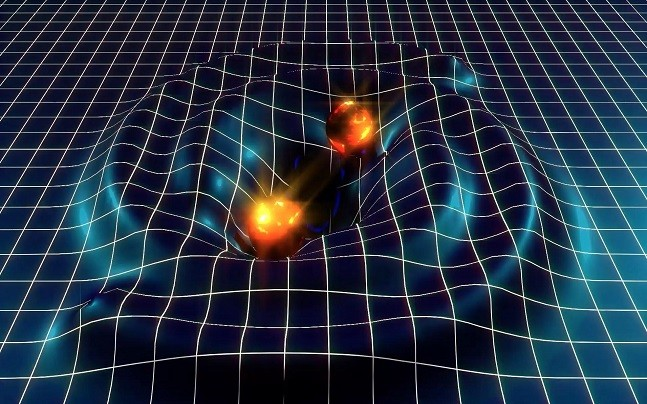
\includegraphics[width=6in]{gwave.jpg}
\caption{A simulation of production of Gravitational waves from binary stars orbiting around each other }
\label{fig:gwave}
\end{center}
\end{figure}      


\subsection{Detection of gravitational waves in LIGO}

LIGO works with the help of two detectors located in the United states. One in Livingston, Louisiana and the other in Hanford, Washington. These detectors are modified Michelson Interferometer with Fabry-Perot cavity introduced to it as shown in Figure \ref{fig:ligosetup}. Each detector is shaped like a gigantic L, in which each arm is 4 Km long. Each arm of the detector forms a Fabry-Perot cavity capped by a semi-transparent Input Test Mass (ITM) and an End Test Mass (ETM). Usually both the arms are of same length. Thus, laser beam takes the same time to travel down each. The interferometer works on the principle of merging of two or more light sources to create an interference pattern. The generated pattern contains information about the object or the phenomenon influencing it. Interferometers can be used to make extremely small measurements that are not achievable using other techniques. 
\vspace{5mm}
\\We now know that Gravitational waves are the ripples formed in the space time. The LIGO interferometers are designed in such a way that when Gravitational Wave pass through Earth, the Interferometer get affected as it makes the detector arms expanded and contracted (the distance between the test masses changes) by as much as 1/10,000 the diameter of a proton.  In Michelson Interferometer, a laser beam passes through a beam splitter resulting in the splitting of the beam into two identical beams separated by a 90-degree angle. Each beam passes through each arms of the Interferometer, get reflected back to the beam splitter from the mirror located at the end of each arm and thus merges back into a single beam at the beam splitter. This produces an interference pattern and will travel towards the photodetector. The photodetector will detect the brightness of the beam falling on it. If both the arms of the Interferometer are of the same length, the beams will travel same distance before recombining and the brightness of the beam detected by the photodetector will be same (constructive interference) as that of the pre-split beam or nothing at all (destructive interference).
\vspace{5mm}
 \begin{figure}[htbp]
\begin{center}
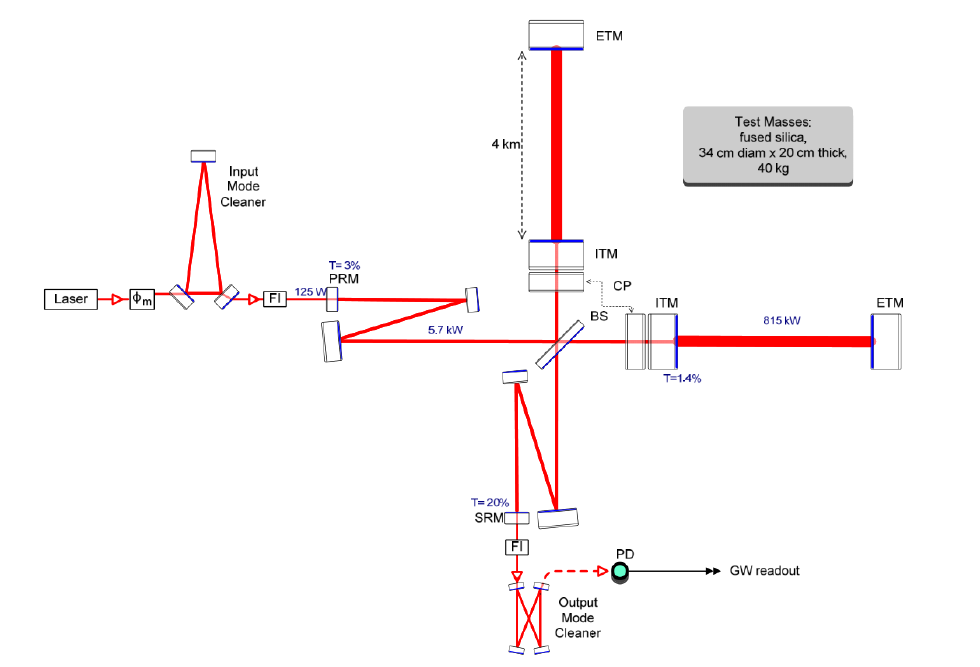
\includegraphics[width=5in]{ligosetup}
\caption{A schematic diagram of the Modified Michelson Interferometer with Fabry-Perot cavity introduced to it }
\label{fig:ligosetup}
\end{center}
\end{figure}   

LIGO interferometers are designed in such a way that no light will fall on the detector as long as the length of the arms are not changing \cite{gwavedetecturl}. No light comes out when the arm lengths are equal but when the arm length change, one beam has to travel farther than the other. Thus, there will be a phase difference between the two beams combining with each other. This causes them to interfere in a different way from they did when they travelled the same distance. As a result, the merged beam will be brighter or dimmer than it was before. In interferometers, the change in light intensity indicates a change in the distance travelled by one or both laser beams. Hence, this interference pattern can be used to make the precise calculation of the change in length occurred and also the nature of the gravitational waves causing this change.

\section{Power losses in the optical setup}
 In the initial LIGO, the interaction time of the Gravitational Waves with each arm of the interferometer is increased by introducing a Fabry-Perot cavity and in order to increase the effective laser power, power recycling has been added \cite{powerloss}. The Advanced LIGO uses the signal recycling techniques to improve the frequency response. As we are dealing with the measurements which are really small, even a fraction of loss in the power of the signal takes away a large set of information and affect the sensitivity of interferometer to Gravitational Waves. Thus, minimising the power loss has always been an important topic of discussion. Different factors that leads to the power loss are listed below in the order of magnitude of their contribution.
 \vspace{5mm}
\\1.Defects \textendash Scattering due to point defects, scratches, sleeks and contamination \textendash loss of 13 ppm per mirror.
\\2.Figure Error of test masses \textendash 24 ppm of combined loss from ITM and ETM.
\\3.Absorption by test mass coatings \textendash loss of 0.5 ppm per mirror.
\\4.Spatial frequency roughness of the test masses \textendash total cavity loss of 7 ppm.
\\5.End Mirror Transmission \textendash Due to Ion beam sputtered coatings \textendash loss of less that 5 ppm.
\vspace{5mm}
\\The round-trip loss of the 4 Km LIGO arm should be made \textless 75 parts per million, in order to make the interferometer effectively sensitive towards Gravitational waves. The main goal of this project is to develop a technique to remove error signals due to the mirror figure error from the interferometer signal in order to get more accurate measurements. This can be done by carefully obtaining a Phase/Mirror map to characterise the mirror surface defects.

\subsection{Mirror figure error in detail}
The LIGO Fabry-Perot Michelson interferometer consists of multiple cavities and thus multiple mirrors. The laser beam is continuously transmitted and reflected from these mirrors. Even though for the mirrors are of high quality, as we go to the scale of 10$^{-19}$ meters we will be able to see some error or discontinuities in the surface of the mirror. These kinds of errors are known as the figure error of the mirror. In other words, we can say that the Mirror figure error is  low frequency surface defects present on the test masses. This results in the low angle scattering of the of the light. The mirror figure error causes power loss in the optical cavities, which ultimately leads to a reduced total power and destruction of squeezed state of light.
\vspace{5mm}
\\Mirror figure error can be characterised by using mirror maps. These diagrams show us the imperfections in the surface of mirror which contribute towards the power loss through scattering. The conventional technique to create these mirror map is Fizeau interferometry. But this cannot be done inside the original LIGO interferometer without disturbing the output. Thus, we are interested in developing a technique which can be used in the original LIGO interferometer. Such techniques are classified as In-situ measurement techniques. 

\subsection{Optical Resonator}
An optical resonator is a system containing two mirrors (ITM and ETM mirrors) separated by a distance. Each arm of the Fabry-Perot interferometer act as an optical resonator. The laser beam passing through each arm bounces back and forth between the mirrors, which leads to the power recycling. Optical resonators are characterised by the radius radii of curvature of the mirrors of the resonator and the absolute distance between them. An optical resonator has a certain set of Hermite-Gaussian modes which are allowed to resonate inside it. All the modes obtained in the transmission spectrum of the Fabry-Perot Michelson interferometer can be expressed as a linear combination of the these eigen H-G modes. Depending upon the characteristic parameter of the resonator and the frequency of the laser, only certain modes will be allowed to resonate inside it. This allows the optical resonator to act as a filter for the laser. The mirrors used in the Fabry-Perot cavity are having extremely small transmittance (=15 ppm) and extremely high reflectance (=1).


\section{Project Proposal: Mode Spectroscopy}
The in-situ technique that we will use in this project is known as the Mode Spectroscopy. In this, we will obtain the transmission spectrum from the interferometer using various techniques. Analyse the data and find the variation of the experimental result from the theoretical expectation with the help of Finesse software. This variation occurs mainly because of the mirror figure error. The shift of the experimental data from the expectation can be used to characterise the source of optical loss in the cavity and thus the shape of the cavity mirror. We are interested in modifying this technique in such a way that it can be used in the 4 Km interferometers. The experiment will be done in the 40 m prototype of the Fabry-Perot interferometer and will be implied to the 4 Km interferometer later.
\vspace{5mm}
\\This project can be divided into three parts.
\\1.	Obtaining the transmission spectrum from the LIGO interferometer.
\\2.	Analysing the data by understanding the shift of the modes from the expectation.
\\3.	Developing a mirror map of the cavity mirrors using the analysis data from step 2.
\vspace{5mm}
\\Each step is discussed in detail below.

\subsection{Step 1: Obtaining the transmission spectrum from the LIGO interferometer }
This can be done by using different methods. Each method has its own advantages and disadvantages. Methods are discussed in detail below. A suitable method will be adapted and it will be used to obtain the transmission spectrum. 
\subsubsection{Cavity Scan}
Cavity scan is a process of feeding a laser of time varying laser frequency to a resonator, in this case to the Fabry-Perot cavity and obtaining the corresponding transmission spectrum. A simple diagram of this kind of setup is shown in Figure \ref{fig:cavityscan} .
\vspace{5mm}
 \begin{figure}[htbp]
\begin{center}
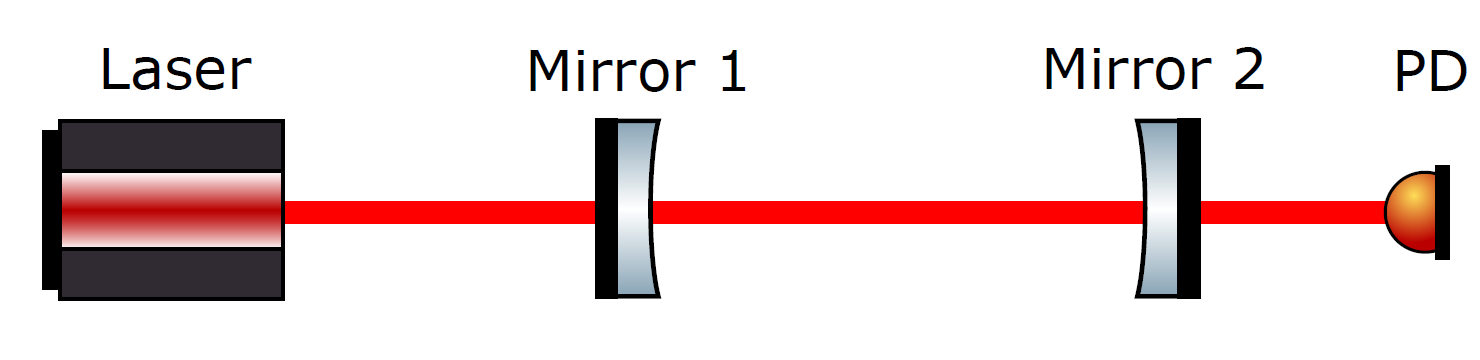
\includegraphics[width=3in]{cavityscan}
\caption{A simple cavity scan setup.}
\label{fig:cavityscan}
\end{center}
\end{figure}
\vspace{5mm}
\\This kind of setup only works if the system is free of any disturbances that might cause the systems to move. Such a system is referred as an Ideally Stable system. The advantage of this method is that it is really easy to execute. But the disadvantage is that no system is exactly stable. Even when a high energy laser falls on the cavity mirrors, it causes the cavity mirrors to move, making it unstable. Also, there are many other factors which makes the system unstable. 
\subsubsection{Using Electric Optical Modulator }
\vspace{5mm}
 \begin{figure}[htbp]
\begin{center}
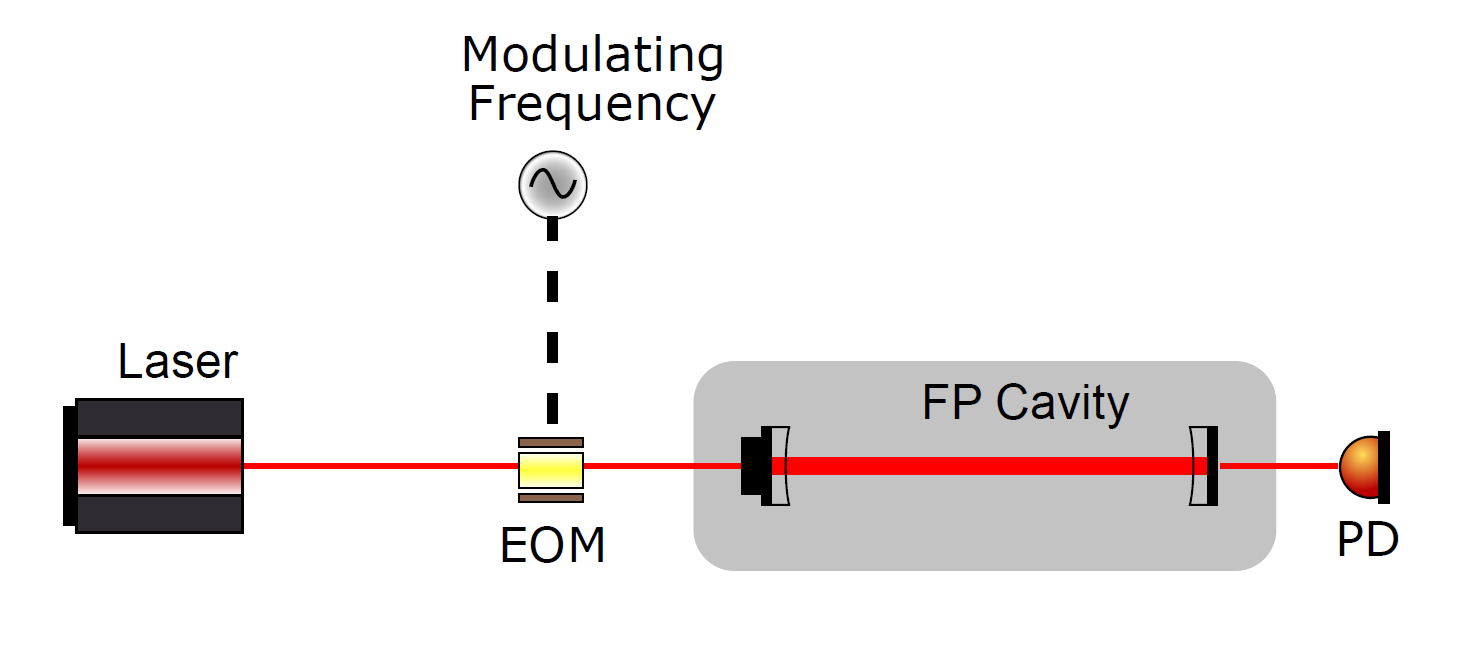
\includegraphics[width=4in]{eom}
\caption{The setup containg EOM to generate sideband frequency}
\label{fig:eom}
\end{center}
\end{figure}
Sideband frequencies are formed using an Electric Optical Modulator (EOM) for a given carrier frequency as shown in Figure \ref{fig:asl}. The main laser is brought in resonance with the cavity. We then vary the side band frequency. This can be used to find the Free Spectral Range (FSR) and the Transverse Mode Spacing (TMS) of the Fabry-Perot cavity .

\subsubsection{Usage of Additional Slave Laser }
In addition to the Master laser used in the Modified Michelson Interferometer, we introduce an additional laser to the setup \cite{alberto}. We call it the slave laser. The Local Oscillator (LO) sets the slave laser as an offset frequency for the Master laser. The relative frequency of the two lasers are kept constant with the help of Phase Locked Loop (PLL). Both the lasers are injected together into the cavity and then cavity is locked with the master laser’s fundamental mode using Pound-Drever-Hall technique. The photodiode connected to ETM detects the intensity of the modes between the lasers. Transmission spectrum is obtained from the spectrum analyser connected to the photodiode. A schematic diagram of this setup is shown in Figure \ref{fig:asl}.
\vspace{5mm}
 \begin{figure}[htbp]
\begin{center}
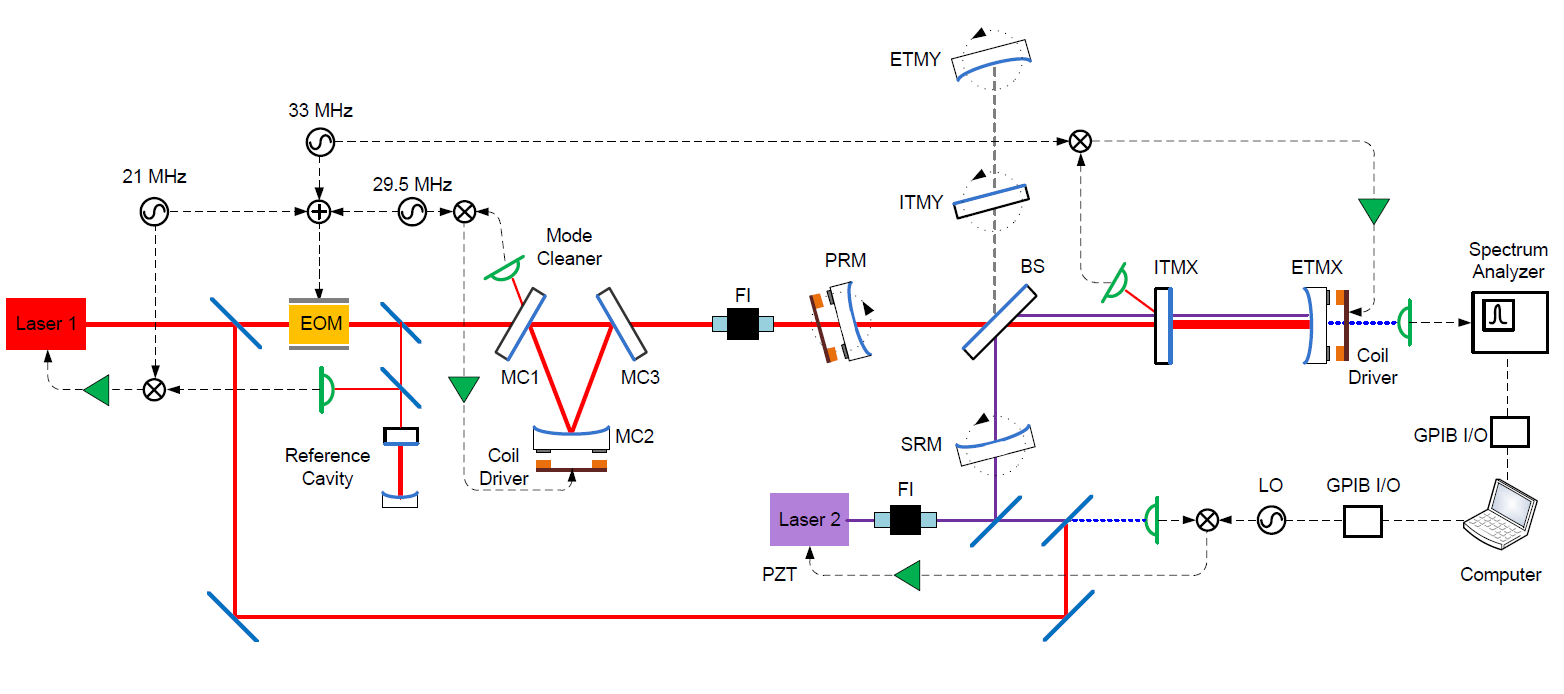
\includegraphics[width=7in]{asl}
\caption{Setup to obtain transmission spectrum using Additional Slave Laser}
\label{fig:asl}
\end{center}
\end{figure}

\subsubsection{Arm Length Stabilization (ALS) Scheme }
In this technique also, we use an additional laser along with the main laser. The additional laser is known as the auxiliary laser and the main laser is known as the pre-stabilised laser (PSL). The auxiliary laser undergoes the process of second harmonic generation (SHG) when it passes through the KDP crystal. As an effect the laser frequency get doubled and wavelength reduces to half. The lasers then travel through the optical systems as shown in the Figure \ref{fig:als}. Finally, by analysing the intensity of auxiliary laser and the PSL we can get the transmission frequency \cite{izumi}.
 \begin{figure}[htbp]
\begin{center}
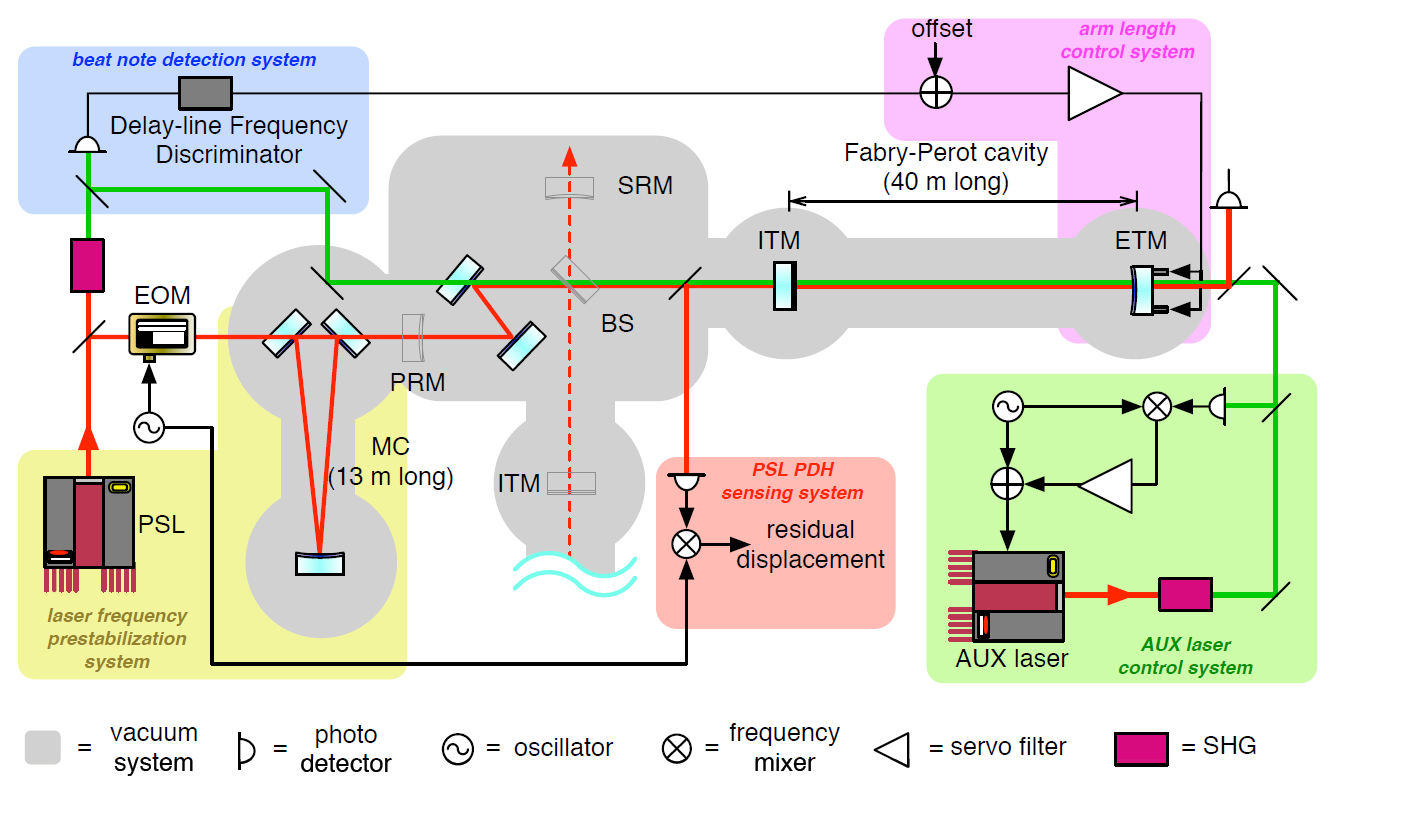
\includegraphics[width=7in]{als}
\caption{Arm length stabilisation setup}
\label{fig:als}
\end{center}
\end{figure}

\subsection{Step 2: Analysing the data by understanding the shift of  modes from the expected spectrum }
Finesse software can be used to simulate an ideal Fabry-Perot cavity with parameters equivalent to that of the 40m prototype of the LIGO interferometer. Frequency input should be provided as a scan and obtain a plot of transmission spectrum. This will allow us to understand the resonant transverse modes of the cavity. This transmission spectrum can be considered as a reference and the transmission spectrum we obtain from the experiment can be compared with this. Any shift of the experimental spectrum from the ideal spectrum should be studied in detail. To make the ideal spectrum more reasonable, sources of errors other than mirror figure error should be considered when we plot the ideal spectrum. Random figure errors are introduced by generating thousands of potential perturbations in the cavity mirror surface with the help of finesse software. By using Monte Carlo Method, the transmission spectrum obtained from the experiment (Step 1) can be written as a linear combination of these potential mirror surface perturbations. This allows us to characterise the sources of optical loss due to mirror figure error.
\subsubsection {Cavity Scan Data and the fitting process}
The cavity scan data is also known as the transmission spectra. The cavity scan contains certain peak resonances. These peaks correspond to fundamental as well as higher order modes (HOM). In order to obtain meaningful parameters from the cavity scan data, we need to perform fitting process. we use Fabry-Perot cavity equations as our fitting model.
 
\subsection{Step 3: Developing a mirror map of the cavity mirrors using the analysis data from step 2 }
Bayesian inference method can be used to predict the probability of each perturbation we developed in step 2. This technique is done by continuously updating the perturbation probability as more details become available. This allows us to isolate the perturbations that are more likely to be present in the cavity. Our ultimate goal is to apply this perturbation probability to the mirror surface and obtain the Mirror Map of the cavity mirrors.

\begin{thebibliography}{9}

 \bibitem{gwaveurl}
       \url{https://www.ligo.caltech.edu/page/what-are-gw}
       
        \bibitem{gwavedetecturl}
       \url{https://www.ligo.caltech.edu/page/ligos-ifo}
 
\bibitem{kaustubh}
     Kaustubh Singhi, Koji Arai and Rana Adhikari
      \emph{''Mirror Metrology using Mode
Spectroscopy'', LIGO-T1700195-v1}
	
	\bibitem{naomi}
    Naomi Wharton, Koji Arai and Rana Adhikari,
      \emph{''Laser Mode Spectroscopy for Mirror Metrology'', LIGO-T1700195-v3}
	
	\bibitem{powerloss}
     G. Billingsley, H. Yamamoto, and L. Zhang,
      \emph{''Characterization of Advanced LIGO Core
Optics''}
 \url{https://dcc.ligo.org/LIGO-P1700029}
	
	\bibitem{gravitational waves}
	  M. Maggiore,
	  \emph{''Gravitational waves''}.
	 Oxford University Press(2008).    
	 
	 \bibitem{alberto}
   Alberto Stochino, Koji Arai and Rana X. Adhikari,
      \emph{''A Technique for In-situ Measurement
of Free Spectral Range and Transverse Mode Spacing of Optical Cavities''.
LIGO DCC No. - P1200048}
      
      \bibitem{izumi}
   Kiwamu Izumi, Koji Arai, Bryan Barr, Joseph Betzwieser, Aidan Brooks, Katrin Dahl,
Suresh Doravari, Jennifer C. Driggers, W. Zach Korth, Haixing Miao, Jameson Rollins,
Stephen Vass, David Yeaton-Massey and Rana X. Adhikari,
      \emph{''Laser Mode Spectroscopy for Mirror Metrology'', LIGO-T1700195-v3}
      
      \bibitem{naomi}
    Naomi Wharton, Koji Arai and Rana Adhikari,
      \emph{''Multi-color Cavity Metrology''.
LIGO DCC No. - P1200019}
      
   
 
\end{thebibliography} %Must end the environment



\end{document} 
